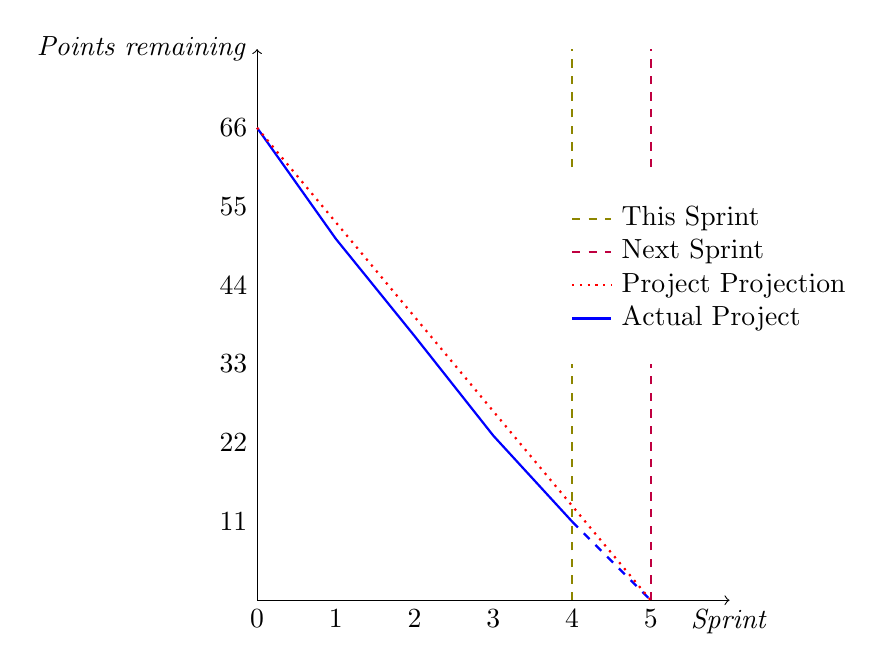
\begin{tikzpicture}

% horizontal axis
    \draw[->] (0,0) -- (6,0) node[anchor=north] {\emph{Sprint}};
% labels
    \draw   (0,0) node[anchor=north] {0}
            (1,0) node[anchor=north] {1}
            (2,0) node[anchor=north] {2}
            (3,0) node[anchor=north] {3}
            (4,0) node[anchor=north] {4}
            (5,0) node[anchor=north] {5};

% vertical axis
    \draw[->] (0,0) -- (0,7) node[anchor=east] {\emph{Points remaining}};
% labels
    \draw   (0,1) node[anchor=east] {11}
            (0,2) node[anchor=east] {22}
            (0,3) node[anchor=east] {33}
            (0,4) node[anchor=east] {44}
            (0,5) node[anchor=east] {55}
            (0,6) node[anchor=east] {66};
    % 1 point is 0.095 
% actual
    \draw[thick, blue] (0,6) -- (1,4.59) -- (2,3.355) -- (3,2.09)-- (4,1.00);
% actual projected
    \draw[thick, dashed, blue] (4,1.00) -- (5,0);

% projected 
    \draw[thick, dotted, red] (0,6) -- (5,0);


% current sprint 
    \draw[thick, dashed, olive] (4,0) -- (4,3);
    \draw[thick, dashed, olive] (4,5.5) -- (4,7);
% next sprint 
    \draw[thick, dashed, purple] (5,0) -- (5,3);
    \draw[thick, dashed, purple] (5,5.5) -- (5,7);


    
\begin{scope}[shift={(4,4)}] 
    \draw[thick, dotted, red] (0,0) -- (0.5,0) 
        node[black, right]{Project Projection};
    \draw[thick, blue, yshift=\baselineskip * - 1] (0,0) -- (0.5,0)
        node[black, right]{Actual Project};
    \draw[thick, dashed, purple, yshift=\baselineskip] (0,0) -- (0.5,0)
        node[black, right]{Next Sprint};
    \draw[thick, dashed, olive, yshift=\baselineskip * 2] (0,0) -- (0.5,0)
        node[black, right]{This Sprint};
\end{scope}

\end{tikzpicture}
